\documentclass[12pt, oneside]{article} 
% \documentclass{article} 
\usepackage{amsmath, amsthm, amssymb, calrsfs, wasysym, verbatim, bbm, 
                color, graphics, geometry}
\usepackage{fancyvrb} % for "\Verb" macro
\usepackage[toc,page]{appendix}
\usepackage[pdftex]{graphicx}
\usepackage{float}
\usepackage{hyperref}
\usepackage{mathtools}


\usepackage{subcaption}

\hypersetup{
    colorlinks=true,
    linkcolor=blue,
    filecolor=magenta,      
    urlcolor=cyan,
}
 
\urlstyle{same}

\geometry{tmargin=1.25in, bmargin=1.25in, lmargin=1.00in, rmargin = 1.00in}  

\newcommand{\R}{\mathbb{R}}
\newcommand{\C}{\mathbb{C}}
\newcommand{\Z}{\mathbb{Z}}
\newcommand{\N}{\mathbb{N}}
\newcommand{\Q}{\mathbb{Q}}
\newcommand{\Cdot}{\boldsymbol{\cdot}}

\usepackage{listings}
\usepackage{color} %red, green, blue, yellow, cyan, magenta, black, white
\definecolor{mygreen}{RGB}{28,172,0} % color values Red, Green, Blue
\definecolor{mylilas}{RGB}{170,55,241}

\title{CIS580 PSet 3}
\author{Sheil Sarda}
\date{02.24.2021}

\begin{document}
\lstset{language=Matlab,%
    %basicstyle=\color{red},
    breaklines=true,%
    morekeywords={matlab2tikz},
    keywordstyle=\color{blue},%
    morekeywords=[2]{1}, keywordstyle=[2]{\color{black}},
    identifierstyle=\color{black},%
    stringstyle=\color{mylilas},
    commentstyle=\color{mygreen},%
    showstringspaces=false,%without this there will be a 
    % symbol in the places where there is a space
    numbers=left,%
    numberstyle={\tiny \color{black}},% size of the numbers
    numbersep=9pt, % this defines how far the numbers are from the text
    emph=[1]{for,end,break},emphstyle=[1]\color{red}, %some words to emphasise
    %emph=[2]{word1,word2}, emphstyle=[2]{style},    
}

\begin{titlepage}
    \begin{flushleft}
        \vspace*{1cm}
        \Huge
        \textbf{CIS580 Problem Set 6\\ }
        \vspace*{0.5cm}
        \normalsize
        Sheil Sarda \verb|<sheils@seas.upenn.edu>| \\
        CIS580 Spring 2021
        \tableofcontents
    \end{flushleft}
\end{titlepage}

\section{Convolution of image with a Gaussian}

\begin{figure}[H]
    \centering
    \begin{subfigure}[b]{0.3\textwidth}
        \centering
        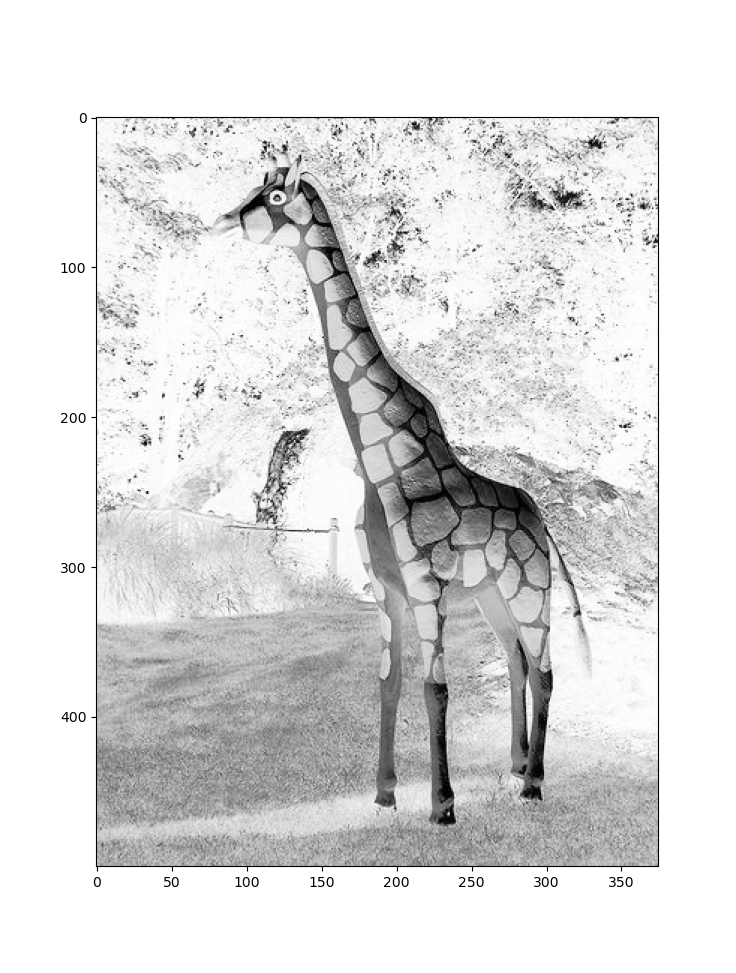
\includegraphics[width=\textwidth]{imgs/q1_original.png}
        \caption{Original Image}
        \label{fig:y equals x}
    \end{subfigure}
    \hfill
    \begin{subfigure}[b]{0.3\textwidth}
        \centering
        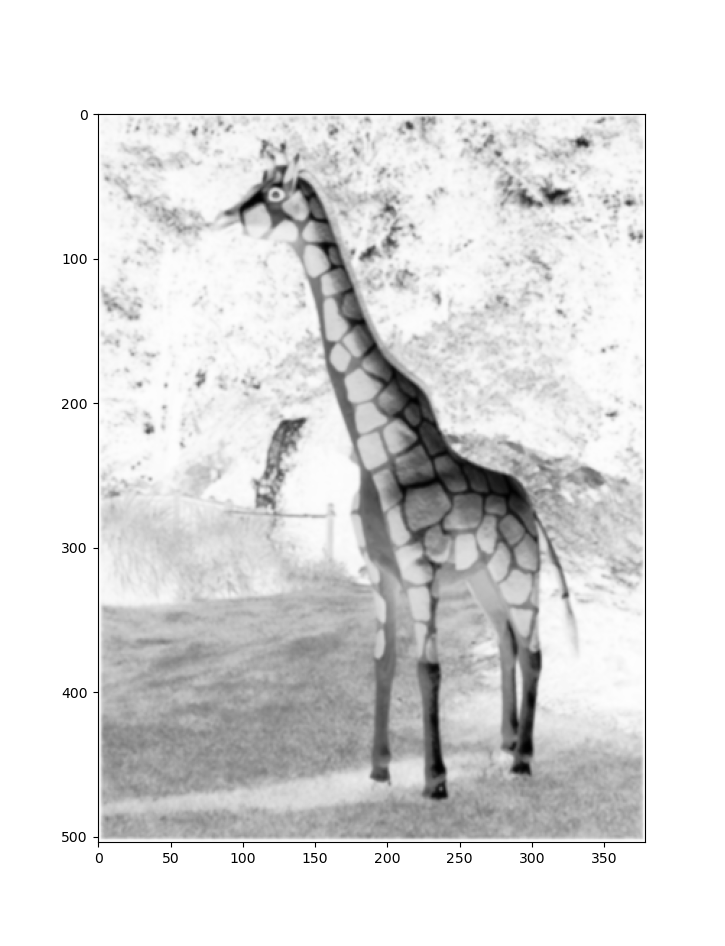
\includegraphics[width=\textwidth]{imgs/q1_plot1.png}
        \caption{$\sigma = 1$}
        \label{fig:three sin x}
    \end{subfigure}
    \hfill
    \begin{subfigure}[b]{0.3\textwidth}
        \centering
        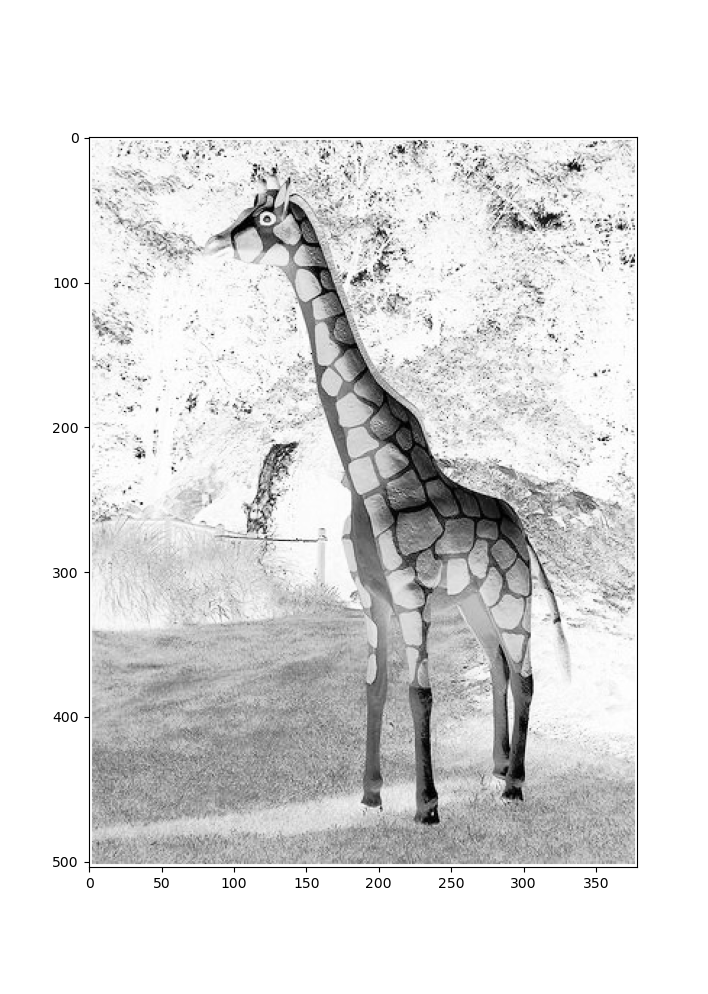
\includegraphics[width=\textwidth]{imgs/q1_plot2.png}
        \caption{$\sigma = 0.1$}
        \label{fig:five over x}
    \end{subfigure}
       \caption{Three simple graphs}
       \label{fig:three graphs}
\end{figure}

The difference between the three images included above is that by increasing 
$\sigma$ from $\sigma = 0$ (original image) to $0.1$ and $1$, we increase the 
Gaussian blur applied to the image. This blurring reduces the image noise and 
detail.


\section{Convolution of Gaussians}

\section{Convolution of Step Edge with Gaussian derivative}


\begin{figure}[H]
    \centering
    \begin{subfigure}[b]{1\textwidth}
        \centering
        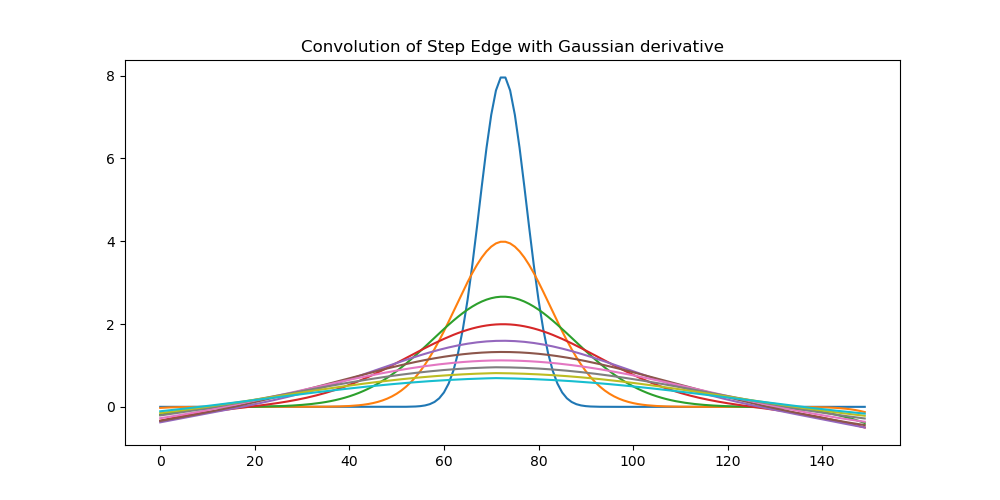
\includegraphics[width=\textwidth]{imgs/q3_plot.png}
    \end{subfigure}
    \caption{}
\end{figure}

\section{Box Function}


\begin{figure}[H]
    \centering
    \begin{subfigure}[b]{1\textwidth}
        \centering
        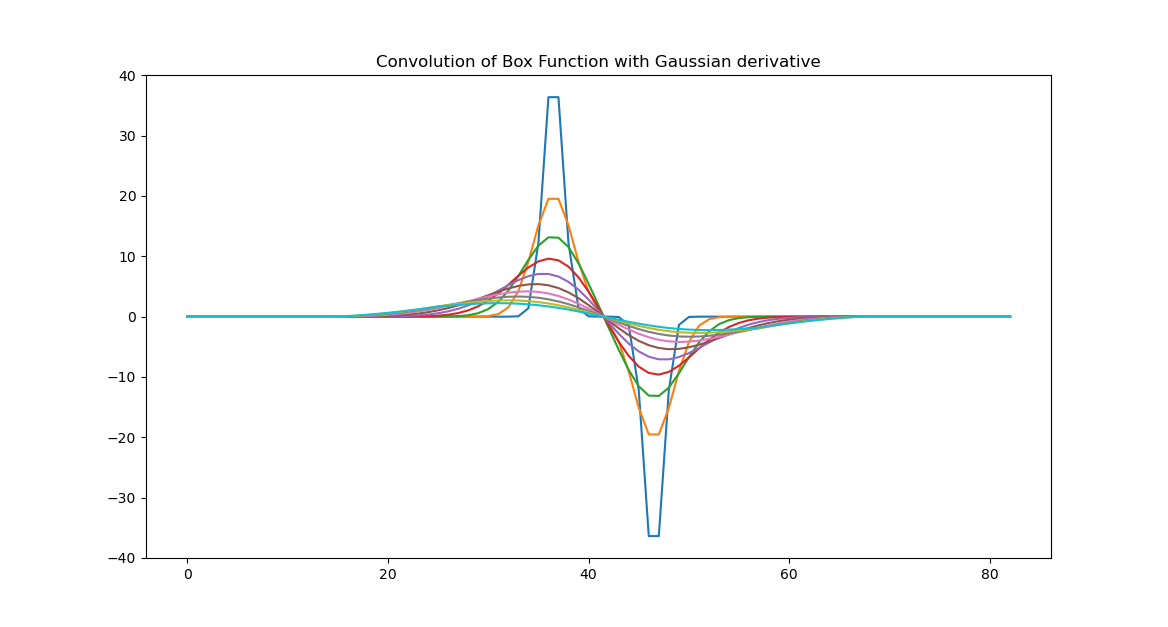
\includegraphics[width=\textwidth]{imgs/q4_plot.png}
    \end{subfigure}
    \caption{}
\end{figure}

\section{1D FFT Quiz}

\begin{figure}[H]
    \centering
    \begin{subfigure}[b]{1\textwidth}
        \centering
        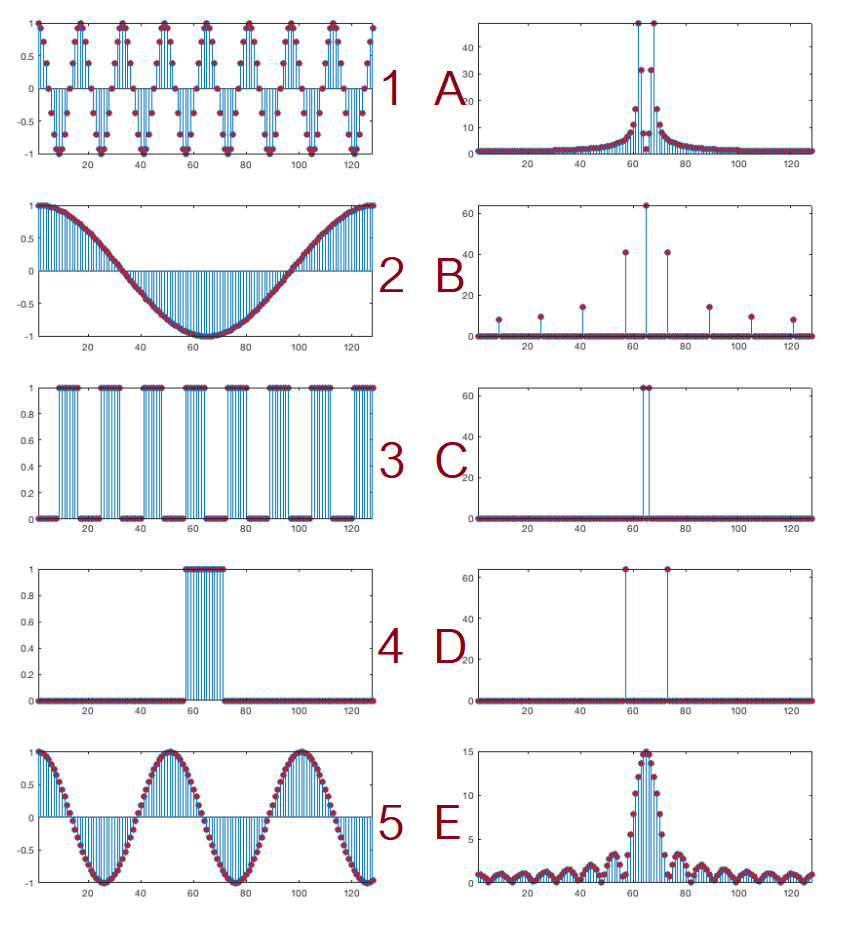
\includegraphics[width=\textwidth]{imgs/q5_matching.png}
    \end{subfigure}
    \caption{}
\end{figure}

\begin{table}[H]
    \centering
    \begin{tabular}{|c|l|}
    \hline
    \multicolumn{1}{|l|}{\textbf{Function}} & \textbf{FFT Plot} \\ \hline
    1                                       & D                 \\ \hline
    2                                       & C                 \\ \hline
    3                                       & B                 \\ \hline
    4                                       & E                 \\ \hline
    5                                       & A                 \\ \hline
    \end{tabular}
\end{table}

My reasoning  for the above matching is that in frequency domain, 
the distance between the two peaks is proportional to the frequency of
the curves.

\section{2D Fourier Transform}


\begin{figure}[H]
    \centering
    \begin{subfigure}[b]{1\textwidth}
        \centering
        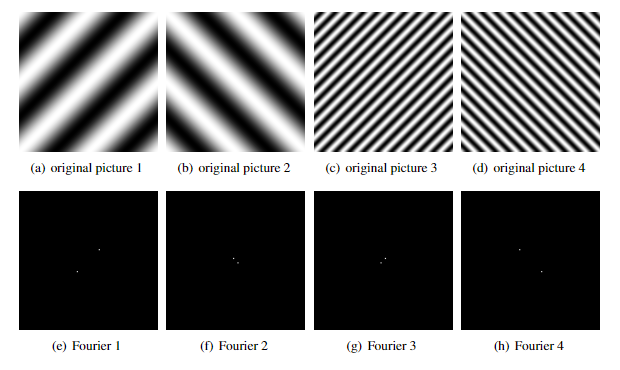
\includegraphics[width=\textwidth]{imgs/q6_matching.png}
    \end{subfigure}
    \caption{Functions and corresponding FFTs}
\end{figure}

\begin{table}[H]
    \centering
    \begin{tabular}{|c|l|}
    \hline
    \multicolumn{1}{|l|}{\textbf{Function}} & \textbf{FFT Plot} \\ \hline
    A                                       & F                 \\ \hline
    B                                       & G                 \\ \hline
    C                                       & H                 \\ \hline
    D                                       & E                 \\ \hline
    \end{tabular}
\end{table}

My reasoning  for the above matching is that the separation of the white dots 
in the frequency domain is proportional to the frequency of the black and white
signals. This reasoning is similar to the 1-dimensional case where 
the distance between the two peaks in the frequency domain was 
proportional to the frequency of the curves.

\section{Filter Design}

\end{document}